%--------------------------------------------
% Chapter: SOFTWARE LAYERS
%--------------------------------------------
\chapter{Software Layer Concept}
\label{sec:layer}

One of the core goals of the layering concept is the maximization of code re-usability. Since major parts of the software is intended to run on multiple platforms, it is mandatory to keep a strict separation between hardware-dependent and hardware-independent software. 

Furthermore, since the hardware is highly modularized, the software shall reflect this modularity as close as possible to ease the interchangeability of sensors. In detail, the modularity encompasses the microprocessor platform (in this project: \texttt{Raspberry Pi B+}) and several extension boards equipped with sensors. In table \ref{tab:layer:hw_sw_comp}, a detailed comparison between hardware modularity and software layering is shown.

To achieve the goal of a maximal code re-usability, the software shall be structured in four general layers (see fig.\ref{fig:layer:layer_graph}). Within each \textbf{\textit{Layer}}, several \textbf{\textit{Functional Units}} are defined in order to divide the software into logically separable modules.
\begin{enumerate}
	\item \textemphs{Application Layer (app)}\\
				This layer contains all high-level software that is necessary for the control of the quadrocopter. Control loops, position hold control, autonomous landing control and supervising functions are here located.
	\item \textemphs{Signal Processing Layer (sig)}\\
				In order to give a flexible framework for filtering and data fusion, a dedicated layer is introduced. The raw sensor data shall be filter (e.g. lowpass filtering). In a second step, the received data shall be fusioned in order to achieve an robust and reliable orientation representation of the quadrocopter.
	\item \textemphs{Hardware Abstraction Layer (hal)}\\
				Since all software of the \texttt{Application Layer (app)} and \texttt{Signal Processing Layer (sig)} shall be system independent, the \texttt{Hardware Abstraction Layer} provides all drivers for the used sensors and extension boards. The interface towards the \texttt{Signal Processing Layer (sig)} will generalize the data flow, independent of the used sensors.\\
				The interfaces towards the \texttt{Low-Level Driver Layer (LLD)} will be called \textbf{Low-Level Driver Interfaces (LLD\_IF)}. These interfaces shall abstract the access the low-level drivers that are usually microprocessor-specific to the used hardware platform (here: Raspberry Pi B+). Thus, all
	\item \textemphs{Low-Level Driver Layer (LLD)}\\
				The \texttt{Low-Level Driver Layer} contains all drivers needed for low-level data communication like \texttt{UART}, \texttt{I2C} or \texttt{SPI}. For the scope of this project (MasterQuad 2015), all needed low-lever drivers are already provided by the chosen operating system.
\end{enumerate}

\begin{figure}[H]
    \centering
    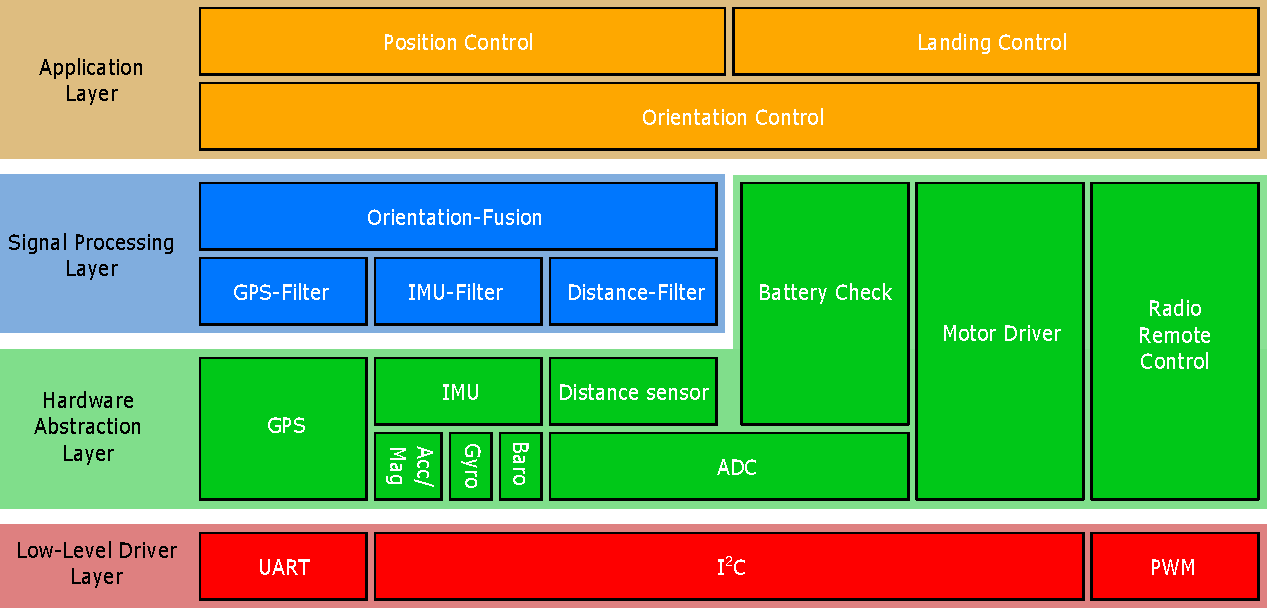
\includegraphics[width=\textwidth]{fig/Software_structure}
    \caption{Software layers with functional units of project MasterQuad 2015}
    \label{fig:layer:layer_graph}
\end{figure}

\begin{table}[H]	
	\begin{tabular}{l|l}
		\hline
		\textbf{Software layer} 					& \textbf{Equivalent interchangeable part} \\
		\hline
		Application Layer (APP) 					& Control loops and supervising/monitoring\\
																			& functions that are usually independent\\
																			& of the used hardware.\\
																			& \textit{\textbf{Example:} GPS-Position Hold functionality}\\
		\hline
		Signal Processing (SIG) 					& \textemphs{Signal conditioning} for used sensors. \\
																			& Additionally for sensor fusion (partly \\
																			& sensor-specific: parameterization of fusion\\
																			& algorithms are usually dependent on the\\
																			& signal/noise properties of sensors).\\
																			& \textit{\textbf{Example:} Kalman-Filter (sensor fusion)}\\			
		\hline
		Hardware Abstraction Layer (HAL) 	& \textemphs{Drivers} for extension boards equipped\\
																			& with sensors for measurements of e.g. \\
																			& acceleration, gyro and distance-to-ground.\\
																			& \textit{\textbf{Example:} GPS-Sensor (extension board)}\\
		\hline
		Low-Level Driver Layer (LLD) 			& Mircoprocessor platform incl. Operating\\
																			& System (if present) and drivers for bus\\
																			& communication (I$^2$C, etc).\\
																			& \textsl{\textbf{Example:} Raspberry Pi B+ Board}\\
		\hline		
	\end{tabular}
	\caption{Comparison between software layers and hardware modularity}
	\label{tab:layer:hw_sw_comp}
\end{table}


%--------------------------------------------
% Chapter: CODE DOCUMENTATION
%--------------------------------------------
\chapter{Code documentation}
\label{sec:doxygen}
For documentation of source code, \texttt{\textemphs{doxygen}} shall be used as an automatic code documentation tool. \texttt{Doxygen} is a special tool that scans C-Files for comments and creates a highly readable documentation in HTML or LaTex. In consequence, this also implies special commenting rules for the coding style guide (see \ref{sec:style:comments}).

\section*{Short guide for doxygen compliant comments}
\label{sec:doxygen:guide}
For every comment that shall be part of the automatic code documentation via \texttt{doxygen}, the respective comment (single line or block) has to be in the line directly above the relevant code. In order to make a comment available to doxygen, the C-comments have to be extended as shown below.\\
Example:
\begin{lstlisting}
//! this is a single line comment (important: '//!' to use doxygen)
unsigned int g_sigGpsfilt_fooStorage_ui32;
\end{lstlisting}

It is also possible to give a short comment in the same line of the relevant code - behind the expression.\\
Example:
\begin{lstlisting}
int g_halAcc_countNr_i32;	//!< doxygen comment in same line as expression
\end{lstlisting}

Both, single line comments and block comments are supported by doxygen.\\
Example:
\begin{lstlisting}
/*! this is a block comment that will be integrated to the code
		documentation, created by doxygen. Similar to C-block comments
		multiple lines are possible. Note the additional exclamation mark 
		in order to get a doxygen compliant block comment!
*/
float g_appLanding_cumquatJuice_f32;
\end{lstlisting}

\textemphs{Important remark:}\\
Only the \textbf{definitions of functions} (\texttt{.c} files) shall be commented in a doxygen compliant manner. The comments of function declarations (\texttt{.h} files) shall only enhance the readability and do not have to be doxygen compliant. All declarations of \textbf{custom data types} or \textbf{global variables} (typically in \texttt{.h} files) are \textbf{mandatory} to be commented in a doxygen compliant manner!

For a more detailed overview of the most important commands to produce a clean doxygen-conform documentation and commenting style, you can have a further look at 
\textbf{
\href{http://www.stack.nl/~dimitri/doxygen/manual/docblocks.html}{Doxygen: Documenting the code} 
}
and 
\textbf{
\href{http://www.stack.nl/~dimitri/doxygen/manual/commands.html}{Doxygen: Special Commands}
}. 
In addition, you can also use the short reference in \texttt{/doc/se/code\_commenting/doxygen\_quickReference.pdf}.
%--------------------------------------------
% Chapter: CODING STYLE GUIDE
%--------------------------------------------
\chapter{Coding style guide}
\label{sec:style}

\section{Naming style}
\label{sec:style:varNaming}
All variables and functions shall have meaningfull names that express the semantic and/or logical use in the code.

It is recommended (but not mandatory) to use the \textbf{Hungarian Notation} (see \href{http://en.wikipedia.org/wiki/Hungarian_notation#Examples}{Wikipedia on Hungarian Notation}). Especially the prefix-postfix notation style is helpful to clarify the scope and data type of the variable's content.

Explicitly forbidden function or variable names are such like \texttt{i}, \texttt{temp}, \texttt{foo}, \texttt{bar}, \texttt{test}, every combination of the given names and all similar words and expressions without descriptive manner.

\subsection{Naming structure for defines \& macros}
\label{sec:style:varNaming:def}

The recommended naming structure for non-local defines (almost all relevant ones) is:
\begin{align}
\texttt{[scope]\_[layer]\_[functionalUnit]\_defName\_[dataType]}
\label{eqn:style:namingStructure}
\end{align}
For strictly local defines, the naming structure may be simplified to the pattern:
\begin{align}
\texttt{[scope]\_defName\_[dataType]}
\label{eqn:style:namingStructure}
\end{align}
Example of recommendation:
\begin{lstlisting}
/*! 
Pattern: 	[global]_[hal]_[gps]_defName_[unsigned 32bit interger] 
*/
#define G_HAL_GPS_HWADDR_UI32;
\end{lstlisting}

All letters of the define/macro name shall be capitals. The \textemphs{scope} and the \textemphs{data type} (only defines) shall be given according to table \ref{tab:style:varNaming:ListOfScopeVar} (table for scope of variables) and table \ref{tab:style:varNaming:ListOfDataType}.

For macros, the data type can be omitted if not necessary.

\subsection{Naming structure for variables}
\label{sec:style:varNaming:var}

The recommended naming structure for non-local variables is:
\begin{align}
\texttt{[scope]\_[layer+functionalUnit]\_varName\_[dataType]}
\label{eqn:style:namingStructure}
\end{align}
For strictly local variables, the naming structure may be simplified to the pattern:
\begin{align}
\texttt{[scope]\_varName\_[dataType]}
\label{eqn:style:namingStructure}
\end{align}
Example of recommendation:
\begin{lstlisting}
/*! 
Pattern: 	[global]_[hal/gps]_varName_[unsigned 32bit interger] 
*/
unsigned int g_halGps_gpsStateNumber_ui32;

/* 
Pattern: 	[local]_varName_[pointer of chars] 
					local pointer on array of ASCII chars
*/
char* l_stringIndex_pch;
\end{lstlisting}

The \textemphs{scope} and \textemphs{data type} of variables shall be given according to table \ref{tab:style:varNaming:ListOfScopeVar} and table \ref{tab:style:varNaming:ListOfDataType}. 

Additionally to the scope and data type, for non-local variables,  the \textbf{hierarchical position} of the variable (\texttt{layer + functionalUnit}) shall be given, as shown in fig.\ref{fig:layer:layer_graph}. The respective layer has to be given first, followed by the name of the functional unit. The layer's name and the functional unit's name shall be separated by a capitalized first letter of the functional unit's name (see example above).

\subsection{Naming structure for functions}
\label{sec:style:varNaming:func}

The recommended structure for function naming is:
\begin{align}
\texttt{[scope]\_[layer+functionalUnit]\_funcName\_[dataType]}
\label{eqn:style:namingStructure}
\end{align}
For strictly local functions (without interface declaration in the header file), the naming structure may be simplified to the pattern:
\begin{align}
\texttt{[scope]\_funcName\_[dataType]}
\label{eqn:style:namingStructure}
\end{align}
The \textemphs{scope} and \textemphs{data type} of functions shall be given according to table \ref{tab:style:varNaming:ListOfScopeFunc} and table \ref{tab:style:varNaming:ListOfDataType}. The data type shall represent the \textemphs{data type of the return variable}.\\
Additionally to the scope and data type, for non-local functions, the hierarchical position of the function (\texttt{layer + functionalUnit}) shall be given, as shown in fig.\ref{fig:layer:layer_graph}. The respective layer has to be given first, followed by a the name of the functional unit separated by a capitalized first letter of the functional unit's name.

Example of recommendation:
\begin{lstlisting}
/* 
	Pattern: 	[local]_[hal/gps]_funcName_[single byte character]
	( remark: the scope of function parameters are given by the literal 'f' 
		        which equals a local scope, but indicates additionally its 
						origin of the parameter list)
*/
char l_halGps_readByte_ch( int f_timeout_i32 );
\end{lstlisting}


\subsection{Literals of scope}
The scope of variables and functions differ in one level of hierarchy. As a consequence, both cases (scope of variables and scope of functions) are shown in detail below to clarify the tiny but relevant differences (see table \ref{tab:style:varNaming:ListOfScopeVar} and table \ref{tab:style:varNaming:ListOfScopeFunc}).

%\subsection*{Scope of variables and the corresponding literals}
\label{sec:style:varNaming:ListOfScope}
\begin{table}[h]
\begin{tabular}{l|l|c}
\hline
\textbf{Scope} 		& \textbf{Scope description}														& \textbf{Literal}\\
\hline
Global						&	The scope of the \textbf{variable} comprises the whole software			&	g\\
(\textbf{variable})				&	and/or the complete layer it belongs to (as shown in  							&	\\
									& fig\ref{fig:layer:layer_graph}).																		& \\
									&	\textit{\textbf{Example:}}																					&	\\
									& \textit{A variable that is used in at least two HAL drivers, e.g.}	&	\\
									& \textit{in \texttt{hal/gps} and \texttt{hal/imu}.}									&	\\
\hline
Module-wide				&	A \textbf{variable} that is used only within a functional unit. The 						& m\\
(\textbf{variable})				& functional unit equals the boxes within one layer, as 				&\\
									&  depicted in fig.\ref{fig:layer:layer_graph}.		&\\
									&	\textit{\textbf{Example:}} 																					&\\
									& \textit{A variable used in at least two functions of the HAL-}			&\\
									& \textit{driver of the GPS sensor.}																	&\\
\hline
Local							&	A \textbf{variable} is local if its scope is strictly limited to the 			& l \\
(\textbf{variable})				& function it belongs to.	A \textbf{special case} are function para-			 			& (f)\\
									& meters (local to the function's body) that shall be denoted					&\\
									& with \texttt{f\_\dots}!																									&\\
									&	\textit{\textbf{Example:}} 																					&\\
									& \textit{A variable declared in the body of a function, or a function}	&\\
									& \textit{parameter.}	&\\
\hline
\end{tabular}
\caption{Literals for the scope of variable naming}
\label{tab:style:varNaming:ListOfScopeVar}
\end{table}

%\subsection*{Scope of functions and the corresponding literals}
\begin{table}[H]
\begin{tabular}{l|l|c}
\hline
\textbf{Scope} 		& \textbf{Scope description}														& \textbf{Literal}\\
\hline
Global						&	A \textbf{function} is global if it shall be callable across the borders	&	g\\
(\textbf{function})				&	  of the layer it belongs to (\textbf{interface between layers}).																		& \\
									&	\textit{\textbf{Example:}}																							&	\\
									& \textit{A function of the HAL Layer shall be callable by a}							& \\
									& \textit{function of the SIG Layer.}					& \\
\hline
Module-wide				&	The scope of a \textbf{function} is module-wide if it	shall be call-		&	m\\
(\textbf{function})				&	 able across the borders of the functional unit	it belongs to.	& \\
									& (\textbf{interface between functional units})														& \\
									&	\textit{\textbf{Example:}}																							&	\\
									& \textit{A function of GPS Filter in SIG Layer (\texttt{sig/gps\_filt})}	& \\
									& \textit{shall be callable by a function of the Orientation Fusion of}		& \\
									& \textit{the same SIG Layer (\texttt{sig/orient\_fusion}).}							& \\
\hline

Local							&	The scope of a \textbf{function} is local if it shall	be callable only	&	l\\
(\textbf{function})	&	  within a single functional unit it belongsto.	No function						& \\
									&   declaration may be given in the header file!													& \\
									&	\textit{\textbf{Example:}}																							&	\\
									& \textit{A function of the GPS driver in HAL shall be callable by}				& \\
									& \textit{another function in the same GPS driver in HAL.}								& \\
\hline
\end{tabular}
\caption{Literals for the scope of function naming}
\label{tab:style:varNaming:ListOfScopeFunc}
\end{table}

\subsection{Literals of data types}
\label{sec:style:varNaming:ListOfDataType}
\begin{table}[H]
\begin{tabular}{c|c|c|c|c}
\hline
\textbf{Data type} 	& \textbf{Size} 	& \textbf{Signedness} & \textbf{C-data type} 							& \textbf{Literal}\\
\hline
integer 						& 8bit 						& signed 							& \texttt{signed char} 							& i8\\
										&  								& unsigned 						& \texttt{unsigned char}						& ui8\\
										& 16bit						& signed 							& \texttt{signed short} 						& i16\\
										&  								& unsigned 						& \texttt{unsigned short} 					& ui16\\
										& 32bit 					& signed 							&	\texttt{signed int}								& i32\\
										&									& unsigned 						&	\texttt{unsigned int}							& ui32\\
										& 64bit 					& signed 							&	\texttt{signed long}							& i64\\
										&									& unsigned 						&	\texttt{unsigned long}						& ui64\\
float 							& 32bit 					& - 									& \texttt{float}										& f32\\
										& 64bit		 				& - 									&	\texttt{double}										& f64\\
boolean							&	-								& -										& (e.g. \texttt{unsigned int})			& bl\\
ASCII byte					& (8bit) 					& - 									&	\texttt{char}											& ch\\
enum 								& - 							&	-										& \texttt{enum strName\{ ... \}}		& en\\
struct 							& - 							&	-										& \texttt{struct strName\{ ... \}}	& st\\
union 							& - 							&	-										& \texttt{union unName\{ ... \}}		& un\\
void 								& - 							&	-										& \texttt{void}											& vd\\
\hline
array 							& - 							&	-										& \texttt{char arrayName[32]}				& rg...\\
\hline
pointers 						& - 							&	-										& dataType\texttt{*}								& p...\\
function pointer		& 32bit (address) &	-										&	-																	& fp\\
\hline
\end{tabular}
\caption{Literals for the data types of variable and function naming}
\label{tab:style:varNaming:ListOfDataType}
\end{table}

\textbf{Pre-allocated arrays}

For pre-allocated arrays, the literal \texttt{rg} (short for 'range') plus the \textbf{size of the pre-allocated array} shall be given.\\
Example:
\begin{lstlisting}
// local pre-allocated array with 255 elements of unsigned 8bit integers
unsigned char	l_myArray_rg255ui8[255];
\end{lstlisting}

\textbf{Pointers}

The literal for \textbf{pointers} is given by \texttt{p}, followed by the literal of the referenced data type (as depicted in table \ref{tab:style:varNaming:ListOfDataType}). Nevertheless, a function pointer is indicated by the fixed literal \texttt{fp}.
Examples:
\begin{lstlisting}
// local pointer on unsigned 8bit integers (e.g. array of 8bit values)
char* 	l_measurementArray_pui8;

// local pointer on ASCII bytes (e.g. string)
char* 	l_measurementArray_pch;

//! global pointer on float (32bit)
float* 	g_appLanding_floatReference_pf32;
\end{lstlisting}


\newpage
\section{Comments}
\label{sec:style:comments}

All code listings of this section can be found in SVN \texttt{/doc/se/code\_commenting} as text files for copy \& paste purposes.

\subsection{Type definitions and non-local variables}
\label{sec:style:comments:typedef}
Type definitions as well as non-local variables (especially enums and structures and unions) shall be declared in the header file of the respective functional unit or layer. Additionally a doxygen-conform commenting is mandatory.

Template with exemplary content:
\begin{lstlisting}[language=C]
/*!**********************************************************************
 * \author 		Juergen Schmidt (juscgs00)
 * \date 			2014/04/01
 * 
 * \brief		Enumeration of all possible GPS sensor states.
 * \details	A detailed descripction about the purpose of the variable 
 *					or typedef. Multiple lines of description is possible. 
 * 					Doxygen will recognize the format automatically.
 * 
 * \internal
 * CHANGELOG:
 * 2015/04/02 olbrgs00:
 * Changed internal blaa production to foo creation
 *
 * \endinternal
 ***********************************************************************/
typedef enum e_gpsStates{
	GPS_UNDEF_EN,             //!< undefined state   
	GPS_INIT_EN,              //!< startup of sensor
	GPS_UNFIXED_SIGNAL_EN,    //!< sensor is searching for satellites
	GPS_FIXED_SIGNAL_EN,      //!< found enough satellites
	GPS_ERROR_EN              //!< non-functional operation
} gpsStatesType;

/*!
	the following line is intentionally commented improperly, since it shall
	only clarify the context of the typedef above. A complete commenting
	block - as depicted for the enum type definition above - would be 
	required for the global variable below!
*/
gpsStatesType g_halGps_opState_en; 
\end{lstlisting}

\newpage
\subsection{Interfaces}
\label{sec:style:comments:functions}
Interfaces (function declarations in \texttt{.h} files) shall be grouped to a reasonable set of interface declarations. Each set shall be commented by the following block. Due to readability, the maximal line width within a block comment shall not exceed 75 characters.

Template with exemplary content:
\begin{lstlisting}
/* -----------------------------------------------------------------------
 * AUTHOR: Juergen Schmidt (juscgs00)
 * DATE OF CREATION: 2014/04/01
 *
 * DESCRIPTION:
 * Interfaces to access all good foos and producting cumquats
 * 
 * CHANGELOG:
 * 2015/04/02 olbrgs00:
 * Changed internal blaa production to foo creation
 * -------------------------------------------------------------------- */
int 	m_halGps_getFooToCumquat_i32(int, float);
int 	m_halGps_SetFooToCumquat_i32(int, float);
int 	m_sigGpsfilt_getCumquatToFoo_int(float, int);
void 	g_sigGpsfilt_updateFooStorage_vd(void);
void 	g_appOrient_updateCumquatStorage_vd(void);
\end{lstlisting}

\subsection{Functions}
\label{sec:style:comments:functions}
Function definitoins, given in \texttt{.c} files, are commented by the following block. Input parameters are numbered in a left to right order. Due to readability, the maximal line width within a block comment shall not exceed 75 characters.

\textemphs{Important remark:}\\
The definitions of functions (\texttt{.c} files) shall be commented in a doxygen compliant manner in order guarantee a comprehensive code documentation!

\newpage
Template with exemplary content:
\begin{lstlisting}[language=C]
/*!**********************************************************************
 * \author 		Juergen Schmidt (juscgs00)
 * \date 			2014/04/01
 * 
 * \brief		Brief description in one line about the function.
 * \details	A detailed descripction about the function, here for creating 
 * 					good foos and much more. Multiple lines of description is
 * 					possible. Doxygen will recognize the format automatically.
 * 
 * \param[in]		f_paramNameOne is a 'call by value' parameter
 * \param[in]	  f_paramNameTwo is a 'call by reference' parameter
 * \param[out]	return value of function
 * 
 * \internal
 * CHANGELOG:
 * 2015/04/02 olbrgs00:
 * Changed internal blaa production to foo creation
 *
 * \endinternal
 ***********************************************************************/
int m_sigGpsfilt_fooCreator_i32(float f_paramNameOne, int f_paramNameTwo)
{
	int l_fooValue_i32;
	int l_cumquatValue_i32;
	
	l_fooValue_i32 			= 22;
	l_cumquatValue_i32 	= 20;
	
	return (l_fooValue_i32 + l_cumquatValue_i32);
}
\end{lstlisting}